The bencharking suite was used to run a number of queries over a varied size
of flow traces. The smallest trace was $500K$ flow records, going upto $10M$
flow records with a step size of $500K$. This accounts for a week worth of
flow data in a university environment. The suite was run on a high-end machine
with $24$ cores of $2.5$ GHz clock speed and $18$GiB of memory. The results
for NFQL and SiLK \footnote{detailed silk installation and usage instructions
are available in the appendix.} \cite{SiLK} are available on the \texttt{benchmarks}
branch of the \texttt{git} repository.

The first query attempts to find all the DNS (over UDP) traffic of the
supplied trace. One of the branch, filters and groups the flow records that
contain DNS requests, while the other holds the DNS responses. The
request-response pairs are then merged according to the endpoints and unfolded
to \marginpar{dns and mdns request-response over udp} display the flow-record
streams in each such pair. Such a query in SiLK \footnote{detailed
instructions to convert flow-tools traces to silk are available in the
appendix} can be represented by piping multiple tools together as shown in
listing \ref{lst:silk-mdns-dns-udp}. The subsequent NFQL query is available at
\texttt{examples/} and is omitted here for brevity reasons. The query is
similar for mDNS whereby the port $53$ is replaced by $5353$. The results are
shown in figure \ref{fig:dns-mdns-udp}.

\lstset{caption=SiLK Query: DNS and mDNS over UDP,
				tabsize=2, language=bash, numbers=left,stepnumber=1,
        basicstyle=\tiny\ttfamily, numberstyle=\ttfamily\color{gray},
        keywordstyle=\color{blue}, frame=shadowbox,
        rulesepcolor=\color{black}, label=lst:silk-mdns-dns-udp,
        aboveskip=20pt, captionpos=b, upquote=true}
\begin{lstlisting}
$ cat dns-udp.txt 
rm -f /tmp/A.raw /tmp/B.raw /tmp/result.raw; \
rwfilter --sport=53 --proto=17 --pass=stdout %s | \
rwsort --fields=sIP,dIP | \
rwgroup --id-fields=sIP,dIP --summarize | \
rwfilter --input-pipe=stdin --pass=/tmp/A.raw --packets=10-; \
rwfilter --dport=53 --proto=6 --pass=stdout %s | \
rwsort --fields=sIP,dIP | \
rwgroup --id-fields=sIP,dIP --summarize | \
rwfilter --input-pipe=stdin --pass=/tmp/B.raw --packets=10-; \
rwmatch --relate=1,2 --relate=2,1 /tmp/A.raw /tmp/B.raw /tmp/result.raw;

$ cat mdns-udp.txt
rm -f /tmp/result.raw; \
rwfilter --sport=5353 --dport=5353 --proto=17 --pass=stdout %s | \
rwsort --fields=sIP,dIP | \
rwgroup --id-fields=sIP,dIP --summarize | \
rwfilter --input-pipe=stdin --pass=/tmp/result.raw --packets=500-; \
\end{lstlisting}

\begin{figure}[ht!]
\centering
\subfigure{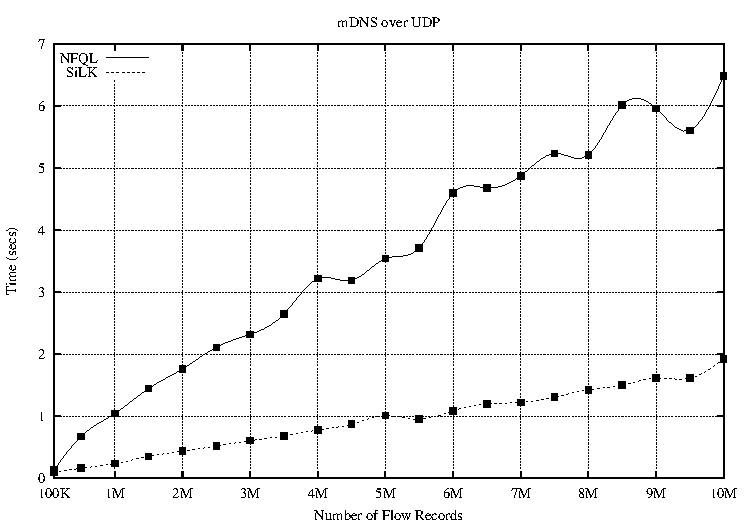
\includegraphics[width=.48\linewidth]{figures/benchmarks/mdns-udp}}\quad
\subfigure{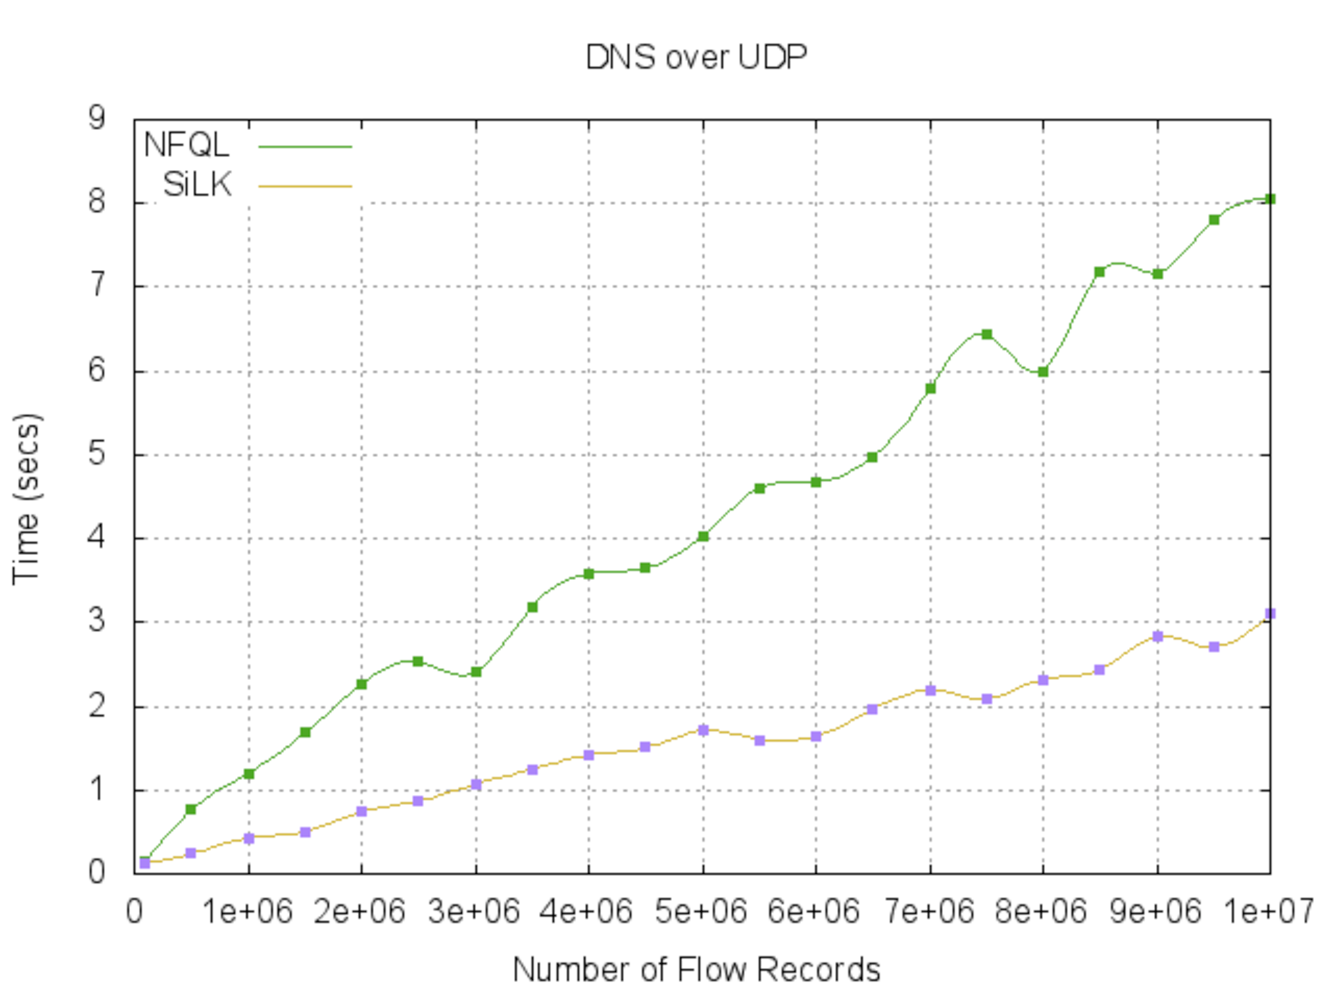
\includegraphics[width=.48\linewidth]{figures/benchmarks/dns-udp}}\\
\caption{F$(v2)$: DNS and mDNS over UDP}
\label{fig:dns-mdns-udp}
\end{figure}


The second query searches for all the HTTP and HTTPs sessions over TCP on a
supplied trace. There are separate branches for requests and responses.
Filters in each such branch search for all HTTP (or HTTPs) traffic over port
$80$ (or $443$). The groupers group all the flow-records with respect to the
endpoints, ie. source-destination IP pairs. The group \marginpar{http and
https sessions over tcp} filters filter the groups to keep only those that
generate at-least 200 packets, while the merger relates the request-response
pairs to create a session. Each such session is then unfolded to display the
stream of flow-records in each session. SiLK queries that tend to emulate the
behavior of findiing HTTP (and HTTPs) sessions is shown in listing
\ref{lst:silk-http-https-tcp}. The comparison results are shown in figure
\ref{fig:http-https-tcp-sessions}.


\lstset{caption=SiLK Query: HTTP and HTTPs Sessions over TCP,
				tabsize=2, language=bash, numbers=left,stepnumber=1,
        basicstyle=\tiny\ttfamily, numberstyle=\ttfamily\color{gray},
        keywordstyle=\color{blue}, frame=shadowbox,
        rulesepcolor=\color{black}, label=lst:silk-http-https-tcp,
        aboveskip=20pt, captionpos=b, upquote=true}
\begin{lstlisting}
$ cat http-tcp-session.txt
rm -f /tmp/A.raw /tmp/B.raw /tmp/result.raw; \
rwfilter --sport=80 --proto=6 --pass=stdout %s | \
rwsort --fields=sIP,dIP | \
rwgroup --id-fields=sIP,dIP --summarize | \
rwfilter --input-pipe=stdin --pass=/tmp/A.raw --packets=200-; \
rwfilter --dport=80 --proto=6 --pass=stdout %s | \
rwsort --fields=sIP,dIP | \
rwgroup --id-fields=sIP,dIP --summarize | \
rwfilter --input-pipe=stdin --pass=/tmp/B.raw --packets=200-; \
rwmatch --relate=1,2 --relate=2,1 /tmp/A.raw /tmp/B.raw /tmp/result.raw;

$ cat https-tcp-session.txt
rm -f /tmp/A.raw /tmp/B.raw /tmp/result.raw; \
rwfilter --sport=443 --proto=6 --pass=stdout %s | \
rwsort --fields=sIP,dIP | \
rwgroup --id-fields=sIP,dIP --summarize | \
rwfilter --input-pipe=stdin --pass=/tmp/A.raw --packets=200-; \
rwfilter --dport=443 --proto=6 --pass=stdout %s | \
rwsort --fields=sIP,dIP | \
rwgroup --id-fields=sIP,dIP --summarize | \
rwfilter --input-pipe=stdin --pass=/tmp/B.raw --packets=200-; \
rwmatch --relate=1,2 --relate=2,1 /tmp/A.raw /tmp/B.raw /tmp/result.raw;
\end{lstlisting}

\begin{figure}[ht!]
\centering
\subfigure{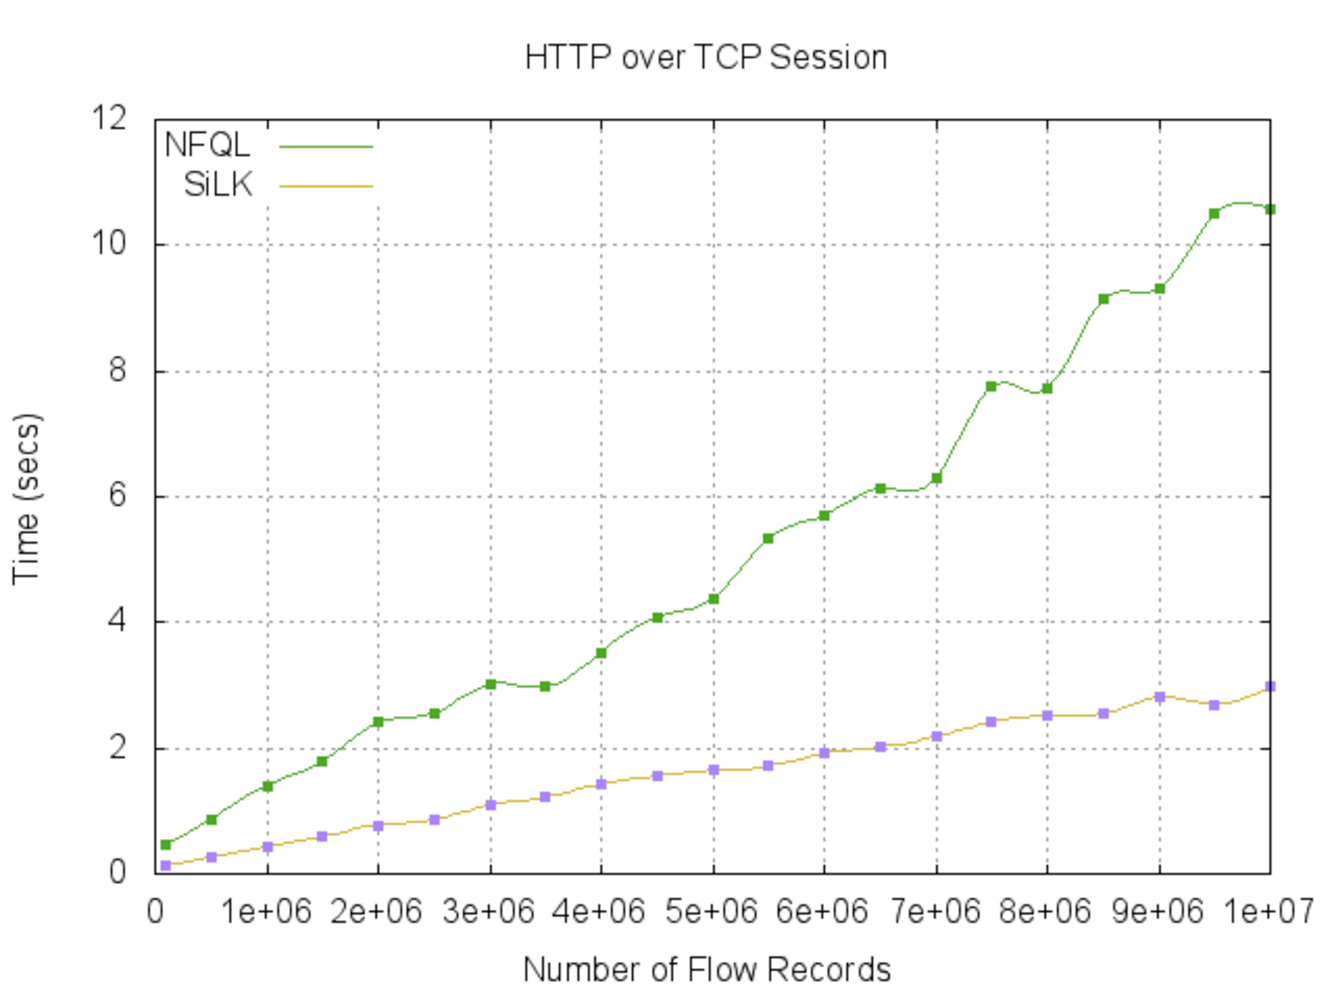
\includegraphics[width=.48\linewidth]{figures/benchmarks/http-tcp}}\quad
\subfigure{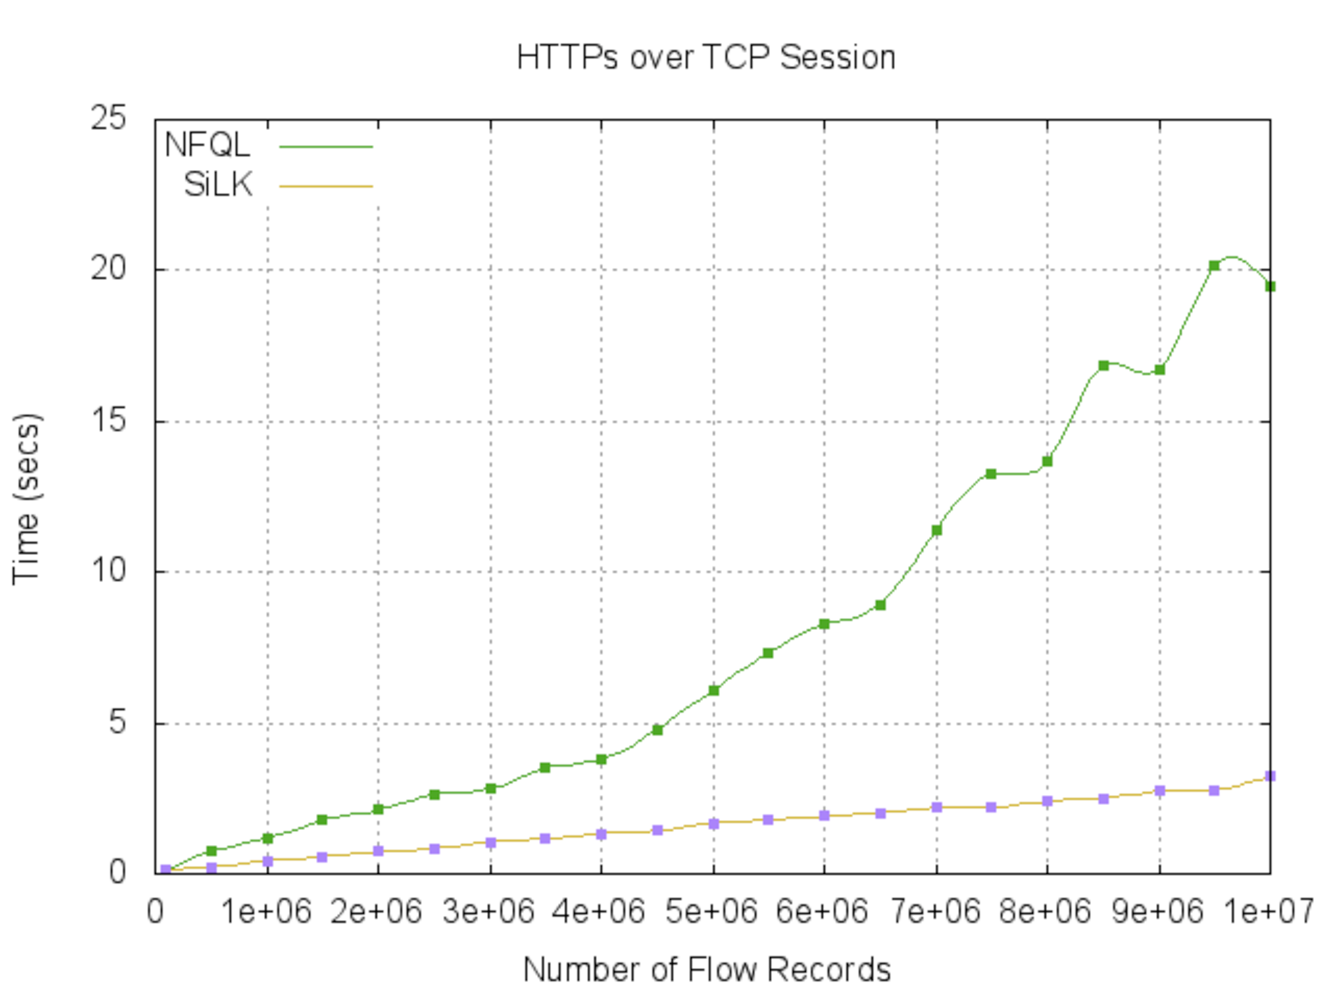
\includegraphics[width=.48\linewidth]{figures/benchmarks/https-tcp}}\\
\caption{F$(v2)$: HTTP and HTTPs Sessions over TCP}
\label{fig:http-https-tcp-sessions}
\end{figure}




The third query attempts to collect an overall statistics of the amount of
HTTP traffic in the supplied flow trace. The two branches represent HTTP
requests and responses. The filters in each such branch, filters in all HTTP
traffic over port $80$. The result from both the branches are
\marginpar{conglomerating http traffic} concatenated together and a sum of all
the packets and octets is generated as a summary. In NFQL such a query is
defined by omitting the grouper module and aggregating all the traffic
generated by the filters.  The merger and ungrouper modules are also omitted.
The SiLK query is shown in listing \ref{lst:silk-http-octets} and the results
are shown in figure \ref{fig:summarizing-http-octets}.


\lstset{caption=SiLK Query: Conglomerating HTTP Traffic,
				tabsize=2, language=bash, numbers=left,stepnumber=1,
        basicstyle=\tiny\ttfamily, numberstyle=\ttfamily\color{gray},
        keywordstyle=\color{blue}, frame=shadowbox,
        rulesepcolor=\color{black}, label=lst:silk-http-octets,
        aboveskip=20pt, captionpos=b, upquote=true}
\begin{lstlisting}
$ cat http-octets.txt
rm -f /tmp/A.raw /tmp/B.raw /tmp/result.raw /tmp/result.txt; \
rwfilter --sport=80 --pass=stdout %s | \
rwfilter --input-pipe=stdin --pass=/tmp/A.raw --packets=0-; \
rwfilter --dport=80 --pass=stdout %s | \
rwfilter --input-pipe=stdin --pass=/tmp/B.raw --packets=0-; \
rwcat --output=/tmp/result.raw /tmp/A.raw /tmp/B.raw; \
rwstats --overall-stats --output-path=/tmp/result.txt /tmp/result.raw
\end{lstlisting}

\begin{figure}[ht!]
\centering
\subfigure{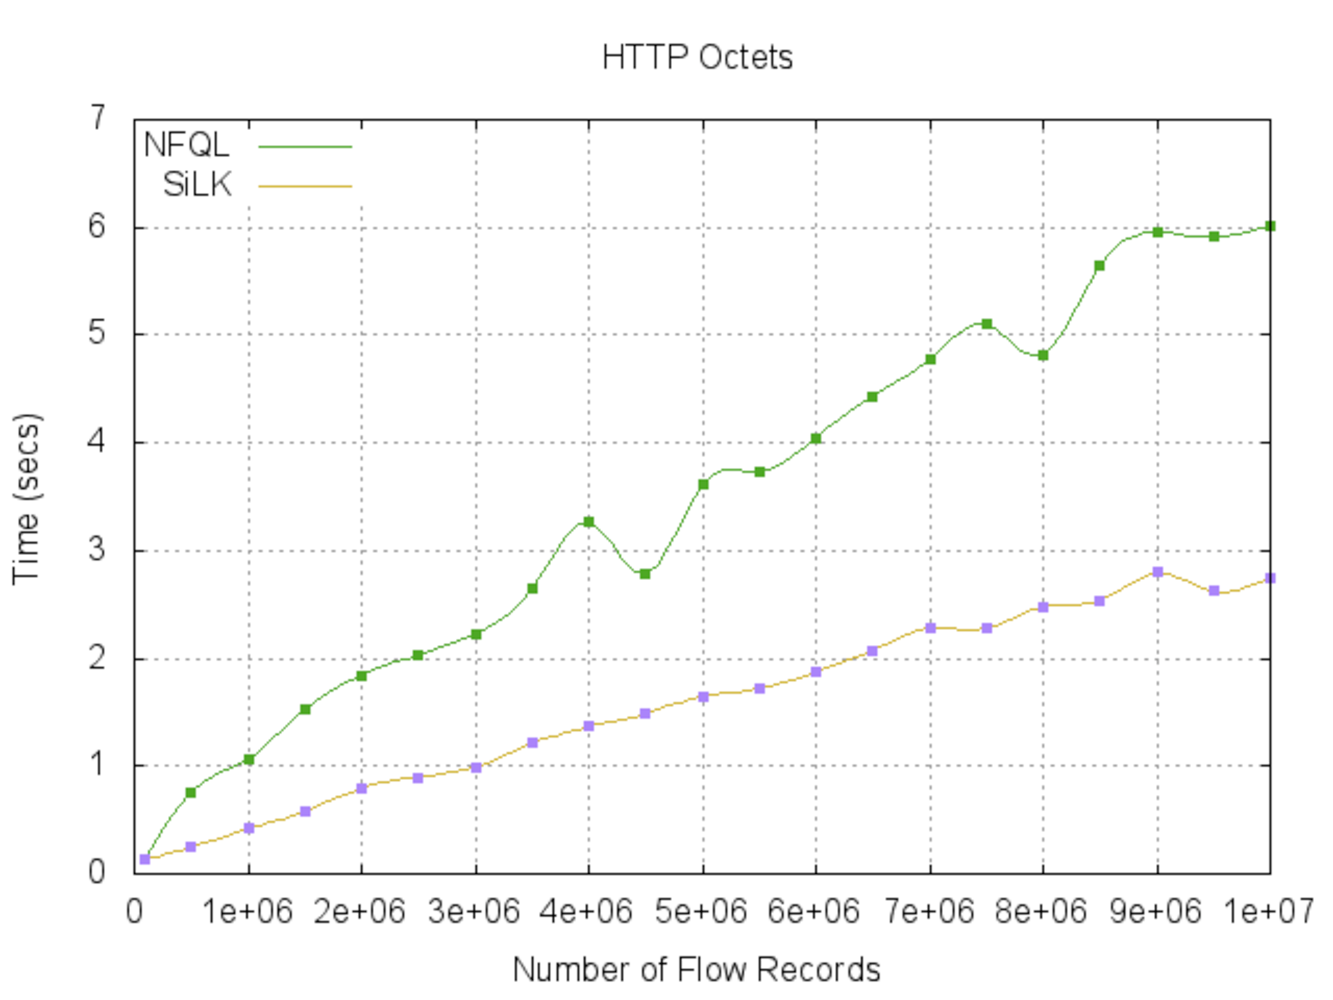
\includegraphics[width=.55\linewidth]{figures/benchmarks/http-octets}}\quad
\caption{F$(v2)$: Conglomerating HTTP Traffic}
\label{fig:summarizing-http-octets}
\end{figure}






The fourth query searches for all application-protocol agnostic TCP sessions
in the supplied trace. The two branches represent TCP requests and responses.
The filters in each branch filter in all the TCP traffic, while the grouper
clubs the flow-records coming to (or from) a specific end-point into one group
record. The group filter, filters in all groups that have at-least $20K$
packets to reduce the merger load. The merger eventually
\marginpar{application agnostic tcp sessions} relates the branches together to
form request-response pairs. The ungrouper unfolds these pairs to print the
stream of flow-records members in each pair. The SiLK query is shown in
listing \ref{lst:silk-tcp-session} and the NFQL comparison results are shown
in figure \ref{fig:tcp-sessions}.


\lstset{caption=SiLK Query: Application Agnostic TCP Session,
				tabsize=2, language=bash, numbers=left,stepnumber=1,
        basicstyle=\tiny\ttfamily, numberstyle=\ttfamily\color{gray},
        keywordstyle=\color{blue}, frame=shadowbox,
        rulesepcolor=\color{black}, label=lst:silk-tcp-session,
        aboveskip=20pt, captionpos=b, upquote=true}
\begin{lstlisting}
$ cat tcp-session.txt
rm -f /tmp/A.raw /tmp/B.raw /tmp/result.raw; \
rwfilter --proto=6 --pass=stdout %s | \
rwsort --fields=sIP,dIP | \
rwgroup --id-fields=sIP,dIP --summarize | \
rwfilter --input-pipe=stdin --pass=/tmp/A.raw --packets=20000-; \
rwfilter --proto=6 --pass=stdout %s | \
rwsort --fields=sIP,dIP | \
rwgroup --id-fields=sIP,dIP --summarize | \
rwfilter --input-pipe=stdin --pass=/tmp/B.raw --packets=20000-; \
rwmatch --relate=1,2 --relate=2,1 /tmp/A.raw /tmp/B.raw /tmp/result.raw;
\end{lstlisting}


\begin{figure}[ht!]
\centering
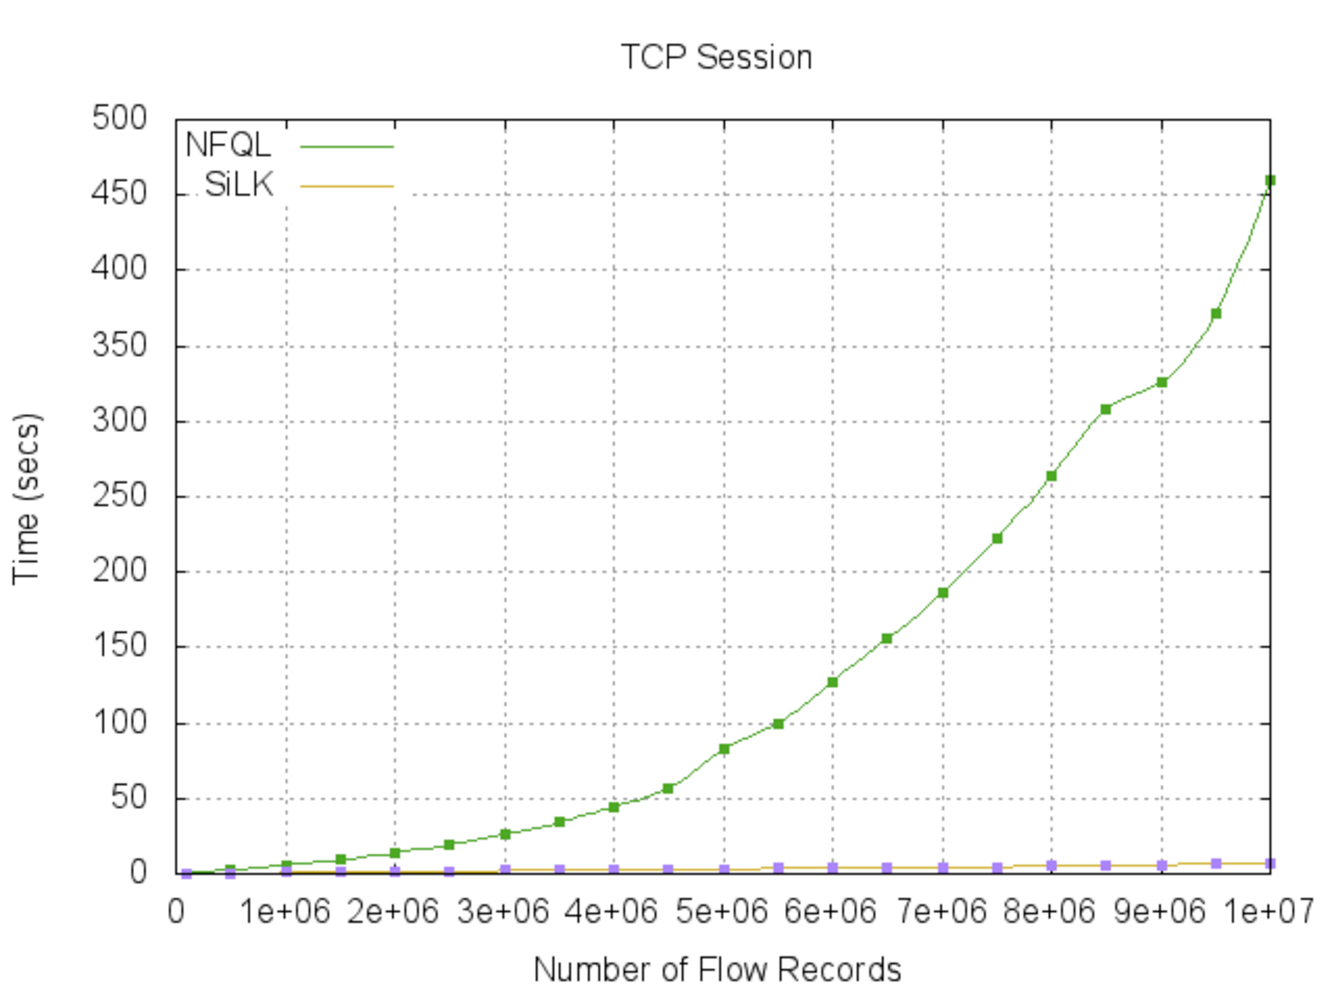
\includegraphics[width=.55\linewidth]{figures/benchmarks/tcp}\\
\caption{F$(v2)$: Application Agnostic TCP Sessions}
\label{fig:tcp-sessions}
\end{figure}

It is clear that the merger is the bottleneck of the processing pipeline. The
near exponential growth is due the $O(n^m)$ complexity of the merger. It
appears that using a hash table for an equality relative operation and search
trees for generic operators will go a long way in improving the merger speed
and is a future work item.
